\documentclass{article}

\usepackage[utf8]{inputenc}
\usepackage[T1]{fontenc}
\usepackage[francais]{babel}
\usepackage{lmodern}
\usepackage{amsthm}
\usepackage{amsmath}
\usepackage{amssymb}
\usepackage{mathrsfs}
\usepackage{verbatim}
\usepackage{moreverb}
\usepackage[top=3cm, bottom=2cm, left=3cm, right=3cm]{geometry}
\usepackage{listings}
\usepackage{graphicx}
\usepackage{hyperref}
\usepackage[boxed,french]{algorithm2e}

\newcommand{\Inde}{\perp \! \! \! \perp}

\lstset{
	basicstyle=\normalsize,
	keywordstyle=\color{blue}, 
	breaklines=true,  
	frame=single,
}


\hypersetup{colorlinks=true, linkcolor=red}

\author{Conrad \bsc{Hillairet} et Alexandre \bsc{Vieira}}
\title{Projet P1 : Statistiques \\ \Large{Approximation Normale de la loi Binomiale Négative}}
\date{\today}

\begin{document}
\maketitle

\setcounter{tocdepth}{4}
\tableofcontents
\newpage

\section*{Introduction}
\addcontentsline{toc}{section}{Introduction} 
En probabilité, on cherche à quantifier l'aléatoire. On définit pour cela plusieurs fonctions, appellées lois de probabilité, qui nous aident à modéliser plusieurs évènements. Il en existe énormément, qui peuvent être à support discret (comme la loi binomiale, la loi de Poisson, ou la loi hypergéométrique) ou à support continu (comme la loi exponentielle, la loi du $\chi^2$ ou la loi Gamma). \\
Le but de ce projet est d'étudier une de ces lois. On s'intéresse ici à une loi à support discret, la loi Binomiale Négative, qu'on peut également appeller loi du n-ième succès. On cherche ici à savoir la probabilité d'arriver au n-ième succès d'une suite d'épreuves de Bernoulli après k épreuves.\\
Ce projet s'intéresse à la modélisation de cette loi informatiquement, et à vérifier l'approche de cette loi par une loi normale.

\bigskip
Ce compte-rendu s'organise de la manière suivante :\\
\begin{itemize}
	\item Un travail mathématique préliminaire sur la loi Binomiale Négative sera présenté, ce qui nous amènera à une idée de la modélisation mathématique faite par la suite.
	\item Cette modélisation, ainsi que ces résultats, seront ensuite exposés et commentés.
	\item La conclusion viendra tout naturellement clore ce rapport.
\end{itemize}



\newpage
\section{Étude mathématique}
\subsection{Préliminaire : loi géométrique}
\begin{enumerate}
\item $X\hookrightarrow \mathcal{G}(p)$ \\
$X(\Omega)=\mathbb{N}^*$\\
La loi de probabilité d'une variable aléatoire suivant une loi géométrique est donnée par :
\[\forall k\in \mathbb{N}^*, \mathbb{P}(X=k)=(1-p)^{k-1} p\]
Vérifions que $\sum_{k=1}^{+\infty} \mathbb{P}(X=k)=1$
\begin{eqnarray*}
\sum_{k=1}^{+\infty} \mathbb{P}(X=k) &=& \sum_{k=1}^{+\infty} (1-p)^{k-1} p \\
				     &=& p \sum_{k=0}^{+\infty} (1-p)^k \\
				     &=& p \times \frac{1}{1-(1-p)} \text{ car }|1-p| <1 \text{ car } p\in]0,1] \\
				     &=& p\times\frac{1}{p} \\
				     &=& 1
\end{eqnarray*}

\bigskip
Nous appelons cela la loi géométrique car le calcul de la série provient du calcul de la série des termes d'une suite géométrique. 

\item Déterminons E(X).
\begin{eqnarray*}
E(X)&=&\sum_{k=1}^{+\infty} k \mathbb{P}(X=k) \\
    &=&\sum_{k=1}^{+\infty} k\times p (1-p)^{k-1} \\
    &=&p\times \sum_{k=1}^{+\infty} k(1-p)^{k-1} \\
    &=&p\times \left( \sum_{k=1}^{+\infty} -(1-p)^k \right)' \text{ car la fonction est continue donc }(1-p)^k\in L^1_{loc} \\
    &=&p\times \left(-(1-p)\times\frac{1}{p}\right)' \\
    &=&p\times\left(-\frac{1}{p}+1\right) ' \\
    &=& p\times\frac{1}{p^2} \\
    &=& \frac{1}{p}
\end{eqnarray*}

\newpage
Déterminons à présent V(X) : 
\begin{eqnarray*}
V(X)&=&E(X^2)-E(X)^2 \\
    &=&\sum_{k=1}^{+\infty} k^2\times p (1-p)^{k-1} - \left(\frac{1}{p}\right)^2 
\end{eqnarray*}
\begin{eqnarray*}
\text{Or, }\sum_{k=1}^{+\infty} k^2\times p (1-p)^{k-1} &=& p \sum_{k=1}^{+\infty} k^2 (1-p)^{k-1} \\
						&=& p \left( -\sum_{k=1}^{+\infty} k (1-p)^k \right) ' \\
						&=& p \left( -(1-p) \sum_{k=1}^{+\infty} k(1-p)^{k-1} \right) ' \\
						&=& p \left( -(1-p) \frac{E(X)}{p} \right) ' \\
						&=& p\left( \frac{p-1}{p^2} \right) ' \\
						&=& p\left( \frac{2}{p^3} - \frac{1}{p^2} \right) \\
						&=& \frac{2-p}{p^2}
\end{eqnarray*}
D'où :
\begin{eqnarray*}
V(X)&=&\frac{2-p}{p^2} - \left(\frac{1}{p}\right)^2 \\
    &=&\frac{1-p}{p^2}
\end{eqnarray*}


\subsection{Étude d'une binomiale négative}
\item Soit $k\in\mathbb{N}^*$. 
\begin{eqnarray*}
\mathbb{P}(Y_n=k)&=&\mathbb{P}(\sum_{i=1}^n G_i =k) \\
		&=& \binom{k-1}{n-1}\mathbb{P}(G_1=k_1 \cap G_2=k_2 \cap ... \cap G_n=k_n)
\end{eqnarray*}
avec $\sum_{j=1}^n k_j = k$. Cela impose que $k_n$ soit combinaison linéaire des autres $k_j$. Ceux-ci peuvent être permutés, d'où le coefficient binomial.
\begin{eqnarray*}
\mathbb{P}(Y_n=k)&=&\binom{k-1}{n-1} \prod_{j=1}^n \mathbb{P}(G_j=k_j) \text{ par indépendance des } G_j\\
		&=&\binom{k-1}{n-1} \prod_{j=1}^n (1-p)^{k_j-1}p\\
		&=&\binom{k-1}{n-1} p^n(1-p)^{\sum_{j=1}^n (k_j -1)} \\
		&=&\binom{k-1}{n-1} p^n(1-p)^{k-n} 
\end{eqnarray*}

\item \begin{eqnarray*}
E(Y_n)&=&E\left(\sum_{j=1}^n G_j\right) \\
      &=&\sum_{i=1}^n E(G_j) \text{ par linéarité de l'espérance }\\
      &=&\sum_{i=1}^n \frac{1}{p} \\
      &=&\frac{n}{p}
\end{eqnarray*}
\begin{eqnarray*}
V(Y_n)&=&V\left(\sum_{i=1}^n G_i\right) \\
      &=&\sum_{i=1}^n V(G_i) \text{ car tous les } G_i \text{ sont indépendants} \\
      &=& \sum_{i=1}^n \frac{1-p}{p^2} \\
      &=& \frac{n(1-p)}{p^2}
\end{eqnarray*}

\item On a supposé que les $G_i$ étaient indépendantes et identiquement distribuées, et du fait de l'espérance et de la variance finie, chacun des $G_i$ est de carré intégrable. On pose $\mu=\mathbb{E}(G_1)$ et $\sigma^2=\mathbb{V}(G_1)$ \\
D'après le théorème limite centrale, on a :
\[\frac{1}{\sigma \sqrt{n}}\sum_{i=1}^n (G_i-\mu) \xrightarrow[n\to+\infty]{\mathcal{L}} N\]
Avec $N\hookrightarrow \mathcal{N}(0,1)$

\bigskip
On peut donc, pour n assez grand, avoir une approximation de $Y_n$ en posant
\[Y_n=\sum_{i=1}^n G_i \approx N'\]
avec $N'\hookrightarrow \mathcal{N}(n\mu,n\sigma^2)$

\item Considérons X qui suit une loi uniforme sur ]0,1[. Si $x$ en est une réalisation, nous pouvons construire une loi de Bernoulli de paramètre p en regardant si $x$ appartient à ]0,p[, dans quel cas nous compterons 1, sinon nous compterons 0. Ce qui en formalisant nous donne : 
		\[Y=1_{]0,p[}(X)\]
avec $X\hookrightarrow \mathcal{U}_{]0,1[}$.\\ On aura alors $Y\hookrightarrow \mathcal{B}(p)$

\item La réalisation d'une variable aléatoire suivant une loi binomiale négative revient à chercher la position du n-ième succès d'une suite d'épreuves de Bernoulli. \\
D'où l'algorithme suivant :\\ 
\begin{algorithm}[H]
	\textbf{entier} n,nbSuccès,position\\
	\textbf{réel} p\\
	\Deb{
	nbSuccès$\leftarrow$0\\
	position$\leftarrow$0\\
	\Tq{nbSuccès<n}{
		\Si{alea()<p}{nbSuccès$\leftarrow$nbSuccès+1}
		position$\leftarrow$ position+1}
	Retourner position
	}
\end{algorithm}
où aléa() est une fonction qui retourne une valeur aléatoire tirée uniformément dans ]0,1[

\end{enumerate}
\section{Résultats du travail de simulation}

Dans cette partie seront présentés les différents résultats de notre travail de simulation.\\
Ce travail consistait à implémenter l'algorithme précédent sous le logiciel Matlab, ce pour un grand nombre de variables. On compare ensuite les résultats obtenus avec la densité de la loi normale pour estimer la véracité de l'approche vue plus haut.

\bigskip
Ces calculs ont été fait pour différentes valeurs de n (1, 5, 10, 20, 50 et 1000) et différentes valeurs de p (0.1, 0.5 et 0.8). Les courbes suivantes présentent un histogramme en fréquence des réalisations de la loi binomiale négative (en bleu) et la représentation de la densité de la loi normale de paramètres $\frac{n}{p},\frac{n(1-p)}{p^2}$ (en rouge).

\bigskip
Pour n=1 : \\
\begin{tabular}{c c}
	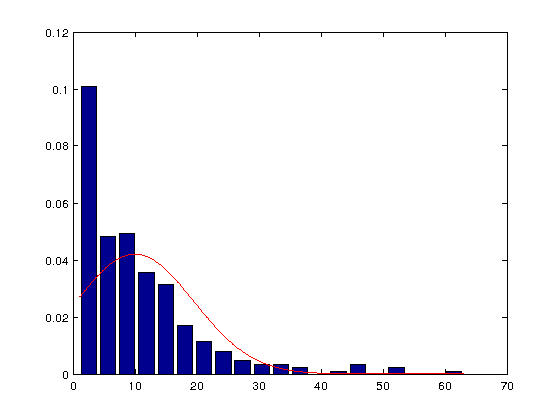
\includegraphics[scale=0.5]{graph/n1p1.png} & 
	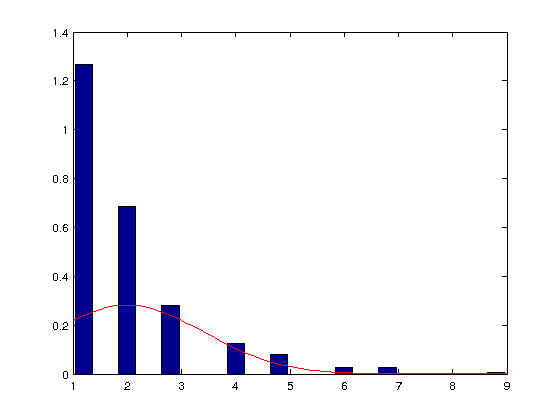
\includegraphics[scale=0.5]{graph/n1p5.png} \\
	p=0,1 &	p=0,5
\end{tabular}\\
\begin{center}
	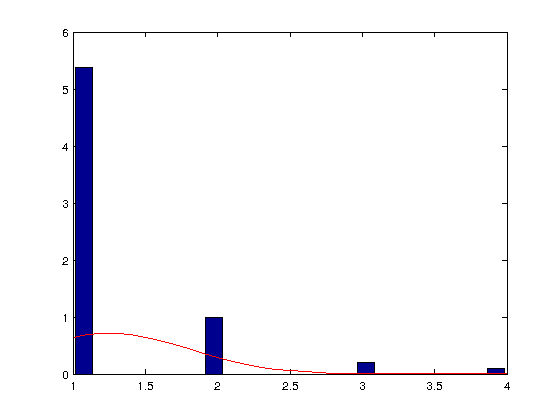
\includegraphics[scale=0.5]{graph/n1p8.png} \\
	p=0,8
\end{center}


Pour n=5 : \\
\begin{tabular}{c c}
	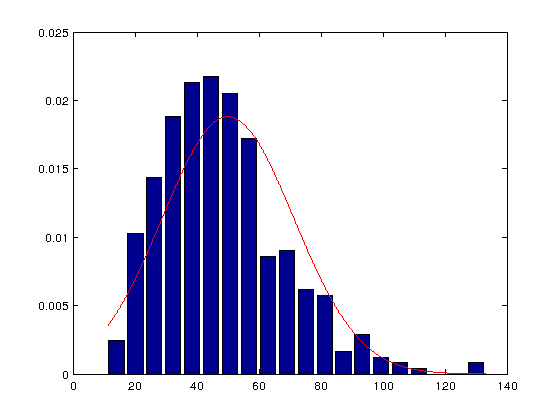
\includegraphics[scale=0.5]{graph/n5p1.png} & 
	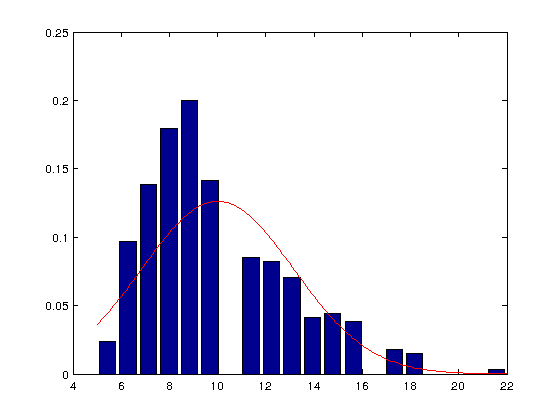
\includegraphics[scale=0.5]{graph/n5p5.png} \\
	p=0,1 &	p=0,5
\end{tabular}\\
\begin{center}
	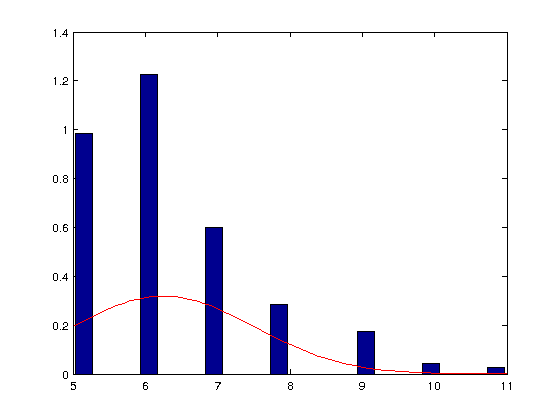
\includegraphics[scale=0.5]{graph/n5p8.png} \\
	p=0,8
\end{center}

\newpage
Pour n=10 : \\
\begin{tabular}{c c}
	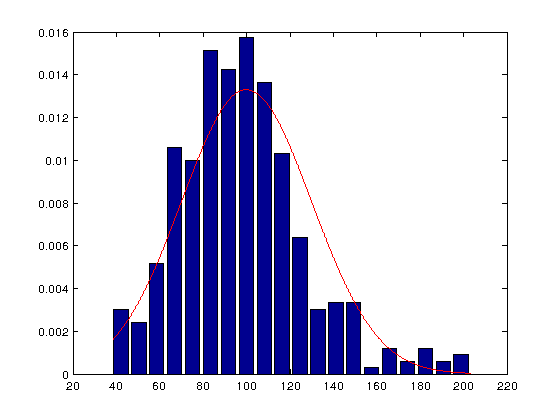
\includegraphics[scale=0.5]{graph/n10p1.png} & 
	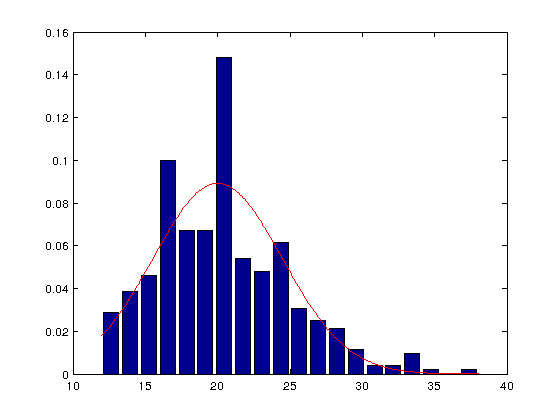
\includegraphics[scale=0.5]{graph/n10p5.png} \\
	p=0,1 &	p=0,5
\end{tabular}\\
\begin{center}
	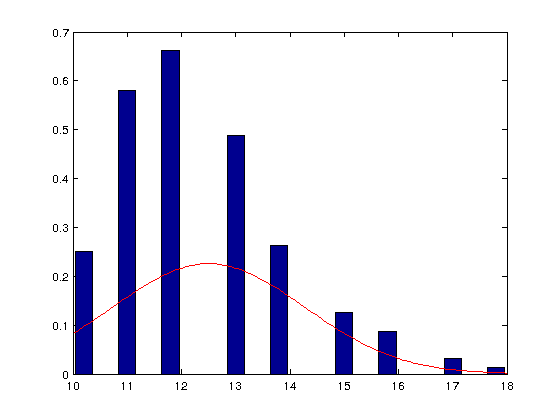
\includegraphics[scale=0.5]{graph/n10p8.png} \\
	p=0,8
\end{center}


Pour n=20 : \\
\begin{tabular}{c c}
	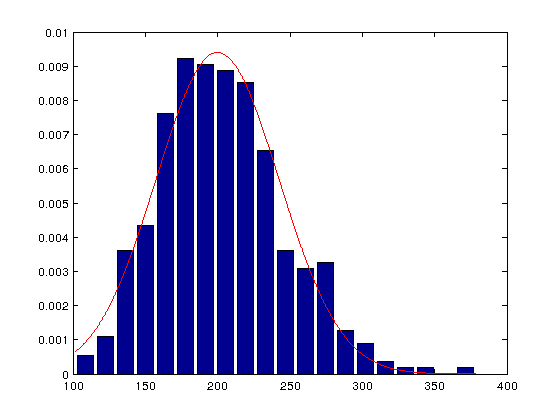
\includegraphics[scale=0.5]{graph/n20p1.png} & 
	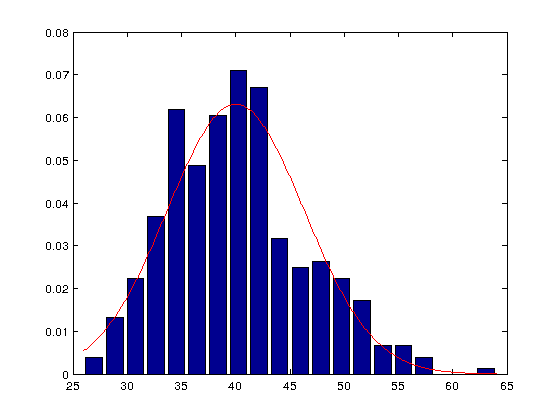
\includegraphics[scale=0.5]{graph/n20p5.png} \\
	p=0,1 &	p=0,5
\end{tabular}\\
\begin{center}
	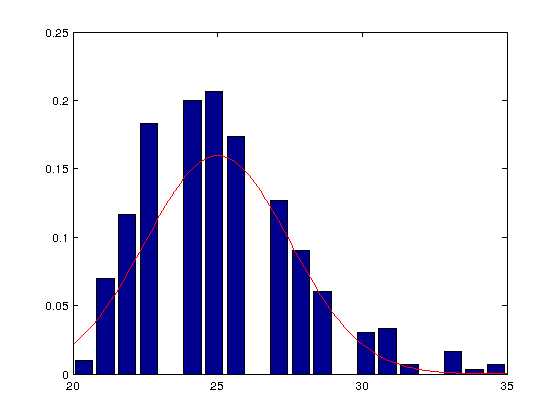
\includegraphics[scale=0.5]{graph/n20p8.png} \\
	p=0,8
\end{center}


Pour n=50 : \\
\begin{tabular}{c c}
	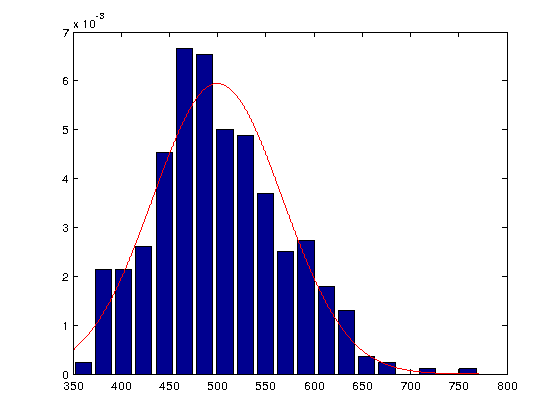
\includegraphics[scale=0.5]{graph/n50p1.png} & 
	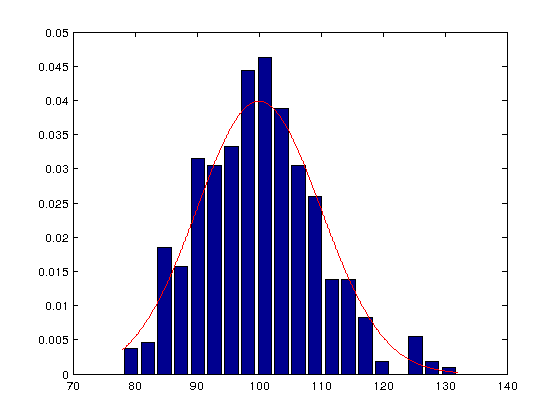
\includegraphics[scale=0.5]{graph/n50p5.png} \\
	p=0,1 &	p=0,5
\end{tabular}\\
\begin{center}
	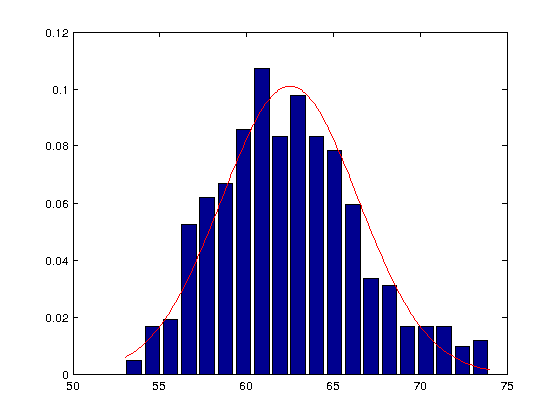
\includegraphics[scale=0.5]{graph/n50p8.png} \\
	p=0,8
\end{center}

\newpage
Pour n=1000 : \\
\begin{tabular}{c c}
	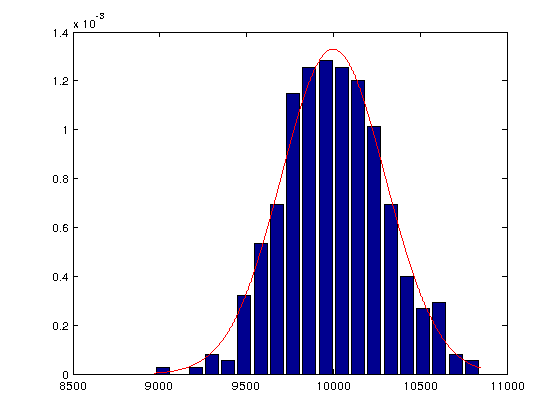
\includegraphics[scale=0.5]{graph/n1000p1.png} & 
	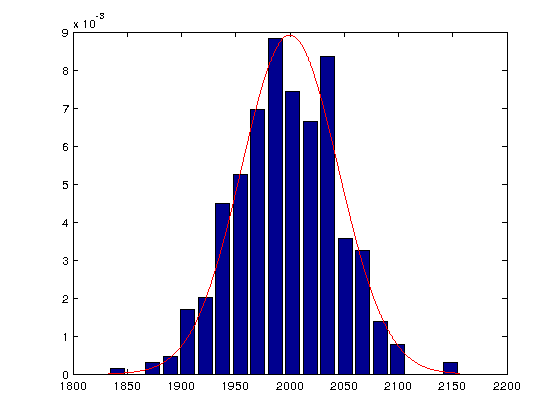
\includegraphics[scale=0.5]{graph/n1000p5.png} \\
	p=0,1 &	p=0,5
\end{tabular}\\
\begin{center}
	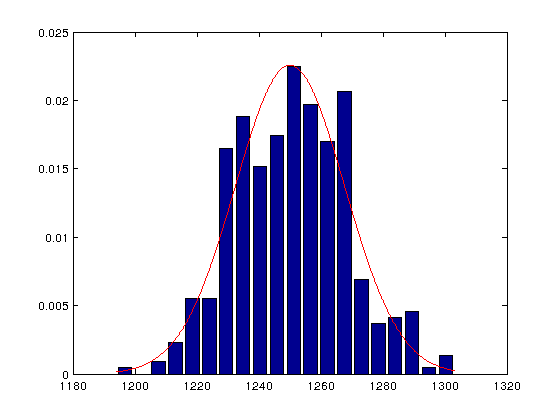
\includegraphics[scale=0.5]{graph/n1000p8.png} \\
	p=0,8
\end{center}

Tout d'abord, on remarque que l'approximation de la loi binomiale négative par une loi normale donne des résultats assez bons dans l'ensemble. Les variations semblent coller dans tous les cas, même si les valeurs ne sont pas toujours les bonnes.

\bigskip
Cependant, on voit très clairement qu'en augmentant la valeur de n, la courbe s'approche de mieux en mieux du diagramme en fréquence, comme on pouvait l'attendre avec le théorème limite centrale. Pour que cette valeur soit bonne pour toutes les valeurs de p testées, on doit tout de même prendre au moins n=50 pour que l'approximation soit assez acceptable. \\
L'approximation dépend donc non seulement de la valeur de n choisie, mais également de la valeur de p. Le couple de paramètres doit donc être bien choisi pour effectuer cette approximation.

\newpage
\section*{Conclusion}
\addcontentsline{toc}{section}{Conclusion} 
Ce projet nous aura permis d'aborder plusieurs problèmes :
\begin{enumerate}
	\item l'étude de la loi Binomiale Négative
	\item l'approche de celle-ci par la loi Normale
	\item la modélisation de ces lois sur ordinateur
\end{enumerate}

On conclut donc que l'approche de la loi binomiale négative par la loi normale est assez bonne, mais qu'il faut prendre garde à prendre des valeurs pour les paramètres qui soient assez probants pour réaliser cette approximation. 

\bigskip
Cette approche peut également se faire pour d'autres lois, comme on l'a fait ici, toujours par le théorème limite centrale. Le tout est de construire une variable comme une somme d'autres variables aléatoires. Les études de ce genre peuvent donc être nombreuses !

\newpage
\section*{Bibliographie}
\addcontentsline{toc}{section}{Bibliographie} 
\noindent \bsc{Lecoutre} Jean-Pierre, \textit{Statistiques et probabilités}, 5ème édition, Dunod, 2012 \\
\bsc{Foata} Dominique, \bsc{Fuchs} Aimé, \textit{Calcul de probabilités}, 2ème édition, Dunod, 1998 \\

\noindent \bsc{de Montigny} S. et \bsc{Le Digabel} S., \textit{Loi normale et théorème central limite}, 2012, 35 slides, disponible \href{http://www.gerad.ca/Sebastien.Le.Digabel/MTH2302D/7_loi_normale.pdf}{ici}

\newpage
\appendix
\section{Annexe}
\subsection*{Code Matlab}
\addcontentsline{toc}{subsection}{Code Matlab}
\lstinputlisting[language=Matlab]{P1Sem2.m}

\newpage
\subsection*{Comparaison avec un autre algorithme}
\addcontentsline{toc}{subsection}{Comparaison avec un autre algorithme}
Comme nous en avons discuté lors de nos différents rendez-vous, un autre algorithme était imaginable pour le calcul de la réalisation d'une variable aléatoire suivant une loi binomiale négative, basé sur la réalisation de plusieurs variables suivant la même loi géométrique.\\
L'algorithme s'articule ainsi :

\begin{algorithm}[H]
	\textbf{entier} i,n,nbSuccès,realBinNeg,realGeo\\
	\textbf{réel} p\\
	\Deb{
	realBinNeg$\leftarrow$0\\
	\Pour{i$\leftarrow$1 à n}{
		realGeo$\leftarrow$1\\
		\Tq{alea()>p}{realGeo$\leftarrow$realGeo+1}
		realBinNeg$\leftarrow$ realBinNeg+realGeo}
	Retourner realBinNeg
	}
\end{algorithm}

\bigskip
Nous avons implémenté un test sous Matlab pour voir si, à chaque fois, le résultat retourné par les deux algorithmes étaient les mêmes ou non. On utilise pour cela la fonction \textit{rng} de Matlab, qui permet de "fixer" les valeurs aléatoires renvoyées par la fonction \textit{rand}. \\
Voici le code de cette implémentation :
\lstinputlisting[language=Matlab]{test.m}

\newpage
Pour différentes valeurs de n et de p, voici les résultats : \\
\begin{tabular}{|c|c|c|c|}
	\hline
	Valeur de n & Valeur de p & Résultat avec le premier algorithme & Résultat avec le deuxième algorithme\\
	 & & (position) & (pos)\\
	\hline
	n=1 & p=0.1 & 10 & 10 \\
	\hline
	n=1 & p=0.5 & 2 & 2 \\
	\hline
	n=10 & p=0.5 & 17 & 17 \\
	\hline
	n=20 & p=0.3 & 37 & 37 \\
	\hline
	n=27 & p=0.65 & 52 & 52 \\
	\hline
	n=42 & p=0.42 & 114 & 114\\
	\hline
	n=100 & p=0.8 & 134 & 134\\
	\hline
	n=300 & p=0.4 & 755 & 755 \\
	\hline
	n=500 & p=0.5 & 971 & 971\\
	\hline 
	n=1000 & p=0.8 & 1 247 & 1 247 \\
	\hline
\end{tabular}

\bigskip
Au vu des résultats, les deux algorithmes ont de fortes chances d'être équivalents.

\end{document}
